\chapter{Ambient Isotopy in $\RR^2$}\label{chap:ambient-isotopy-in-r2}
% \setlength\epigraphwidth{.85\textwidth}
% \epigraph{``Now stop!'' Max said and sent the wild things off to bed\\
%   without their supper. And Max the king of all wild things was lonely\\
%   and wanted to be where someone loved him best of all.}{---Maurice
%   Sendak, \emph{Where the Wild Things Are}}

\setlength\epigraphwidth{.7\textwidth}
\epigraph{Then all around from away across the world\\
  he smelled good things to eat\\
  so he gave up being king of where the wild things are.\\
  But the wild things cried, "Oh please don't go --\\
  we'll eat you up --- we love you so!"\\
  And Max said, ``No!''}{---Maurice Sendak, \emph{Where the Wild
    Things Are}}


% To that end, we show that \emph{all} knots in $\RR^2$ are ambient
% isotopic to each other (no PL condition needed). Most sources list
% this as a direct consequence of the Jordan-Schoenflies theorem
% (\cref{thm:jordan-schoenflies}); however, we could not find an
% argument that we found detailed enough to be satisfying. Hence we give
% our own proof. This introduces some of the machinery we'll apply to
% the $\RR^3$ case (particularly some results about the extent to which
% we can isolate strands of a general topological embedding from each
% other), and will also provide an opportunity for us to introduce the
% notion of \emph{feral} points.

%     \emph{Feral points} are points in the image of an embedding $K$ where
%     $K$ is highly ``oscillatory,'' as defined by a local transformation to
%     a polar parameterization of $K$. Feral points represent a sort of
%     ``boundary'' to wildness. Every wild point is a feral point, but not
%     every feral point is a wild point. This explains the confusion with
%     the countable Reidemeister I move example the we alluded to in the
%     preface. There, the point of convergence for the loops was a
%     \emph{feral} point for the diagram, which captures the idea of why it
%     looks ``wild'' at first glance.


We will now examine how ambient isotopy behaves in $\RR^2$. Our main
goal is to show that in $\RR^2$, \emph{all} embeddings are ambient
isotopic. The motivation is to use this result to show that in
$\RR^3$, for two curves $\gamma_1, \gamma_2$ embedded in a compact
neighborhood $V \subseteq \RR^3$ such that $\gamma_1$, $\gamma_2$
share the same endpoints, then if $\gamma_1, \gamma_2$ have no
crossing points in the diagram given by some projection map $\pi$,
then $\gamma_1$, $\gamma_2$ are ambient isotopic by an ambient isotopy
fixing $\partial V$. This will be useful later when we attack the
problem of determining which wild knots can be represented by a
countable union of polygonal segments.

To that end, we must first discuss the extent to which we can separate
distinct strands of a knot by closed neighborhoods. This will allow us
to modify our knots locally by considering ambient isotopies in these
neighborhoods that fix the boundaries. Then, we will be able to apply
\cref{thm:uniformly-convergent-ambient-isotopy} or
\cref{thm:countable-gluing-ambient-isotopies} to combine all of these
into a \emph{single} ambient isotopy achieving our desired effects.


% \section{Some Useful Results}
% To go further in studying arbitrary topological embeddings, we need be
% able to partition our embedded knot into (possibly infinitely-man)
% pieces that we can control the local behavior on. As such, we'll need
% to start incorporating some machinery from Analysis. We'll prove some
% technical results about separating strands, and use these to examine
% the relationship between orientatin-preserving homeomorphism and
% ambient isotopy in $\RR^2$. In particular, we'll see that we can drop
% the PL condition and just treat the two like they're the same thing.
% We expect a similar result holds in $\RR^3$, but due to time
% constraints, we were not able to explore the topic.





% We will make use of this in $\RR^3$ by using it to show that
% if a knot has a $2$D projection with
% that \emph{all} embeddings
% in $K : S^1 \into \RR^2$ are ambient homeomorphic.\footnote{Of course,
%   all $K : S^0 \into \RR^2$ are ambient homeomorphic as well, by a
%   simple translation map.} The second gives us some basic
% characterizations of tameness for $K : S^1 \into \RR^3$.
\section{All Embeddings in $\RR^2$ are Ambient Isotopic}
We begin by recalling the Jordan-Schoenflies
theorem:\footnote{Pronunciation guide: \ipa{ZO\;Rd\~a} and \ipa{"S\o
    :nfli:s}, respectively.}
\begin{theorem}[Jordan-Schoenflies]\label{thm:jordan-schoenflies}
  Let $\gamma : S^1 \to \RR^2$ be a simple closed curve, and let
  $\iota : S^1 \into \RR^2$ be the standard inclusion of $S^1$ as the
  unit circle. Then there exists a homeomorphism $f : \RR^2 \to \RR^2$
  such that $f \circ \gamma = \iota$.
\end{theorem}
Note, ``simple closed curve'' is equivalent to ``embedding.'' We just
chose ``simple closed curve'' to match the language commonly used when
stating the theorem. Anyways, the following is an immediate corollary:
\begin{corollary}[All Embeddings in $\RR^2$ are Ambient
  Homeomorphic.]\label{cor:all-embeddings-in-r2-ambient-homeomorphic}
  Let $K_0, K_1 : S^1 \into \RR^2$. Then $K_0$ and $K_1$ are ambient
  homeomorphic.
\end{corollary}
\begin{sproof}
  By Jordan-Schoenflies, there exist ambient homeomorphisms $f_0, f_1
  : \RR^2 \to \RR^2$ such that $f_0 \circ K_0 = \iota = $ and $f_1 \circ
  K_1 = \iota$. Hence
  \begin{align*}
    (f_1^{-1} \circ f_0) \circ K_0
    &= f_1^{-1} \circ (f_0 \circ K_0) \\
    &= f_1^{-1} \circ \iota \\
    &= f_1^{-1} \circ (f_1 \circ K_1)  \\
    &= K_1. \qedhere
  \end{align*}
\end{sproof}
We now show the main result: In $\RR^2$, ambient
orientation-preserving homeomorphism is equivalent to ambient isotopy.
Again, we know this holds in the PL case, but were unable to find a
proof for the topological case. First, we have the following:
\begin{lemma}\label{lem:polygonal-curves-are-equivalent}
  Let $K_0, K_1 : S^1 \into \RR^2$ be simple polygonal curves. Then
  $K_0, K_1$ are ambient isotopic by some $F : [0,1] \times \RR^2 \to
  \RR^2$ such that for some compact set $V$, $F$ is identity on $[0,1]
  \times (\RR^2 \setminus V^\circ)$.
\end{lemma}
\begin{sproof}
  This follows as a consequence of an argument similar to those given
  in \cref{sec:rigorous-ambient-isotopy}. In particular, see
  \cref{cor:moving-through-simplices}
\end{sproof}
Our goal is to take finer and finer polygonal approximation of $K$,
using \cref{lem:polygonal-curves-are-equivalent} to argue ambient
isotopy with the unit circle, and taking a limit to obtain the result.
There is a problem that we need to be mindful of, though: If we aren't
careful, naively connecting subsequent points together with straight
lines will introduce crossings, which would prevent us from applying
\cref{lem:polygonal-curves-are-equivalent}. Our strategy will be to
use \cref{thm:separating-strands} to separate the strands of our knot
from each other, and then use the lemma below to connect the endpoints
of these strands by an $\varepsilon$-close polygonal approximation.
\begin{lemma}\label{lem:polygonal-path-connected}
  Let $X \subseteq \RR^n$ be open and connected. Then $X$ is
  polygonally path-connected.\footnote{I.e., every two points are
    connected by a finite sequence of line segments.}
\end{lemma}
\begin{proof}
  Let $x_0 \in X$ be arbitrarily chosen. We want to show that $x_0$ is
  polygonally path connected to every other point of $X$. To that end,
  define $C_{\rm poly}$ by
  \[
    C_{\rm poly} = \set{x \in X \MID \text{ there exists a finite
        polygonal path in $X$ from $x_0$ to $x$}}.
  \]
  Note that $C_{\rm poly}$, $C_{\rm poly}^c$ partition $X$. We claim
  $C_{\rm poly}$ is clopen.
  \begin{itemize}
    \item ($C_{\rm poly}$ is open): Let $x_1 \in C_{\rm poly}$ be
      arbitrarily chosen. Then by definition, there exists a polygonal
      path $P_{0,1}$ from $x_0$ to $x_1$. We'll use this later.

      Now, since $X$ is open, there exists $\varepsilon > 0$ such that
      $B_{\varepsilon}(x_1) \subseteq X$. We want to show
      $B_{\varepsilon}(x_1) \subseteq C_{\rm poly}$. To that end, let
      $x_2 \in B_{\varepsilon}(x_1)$ be arbitrary, and bserve that the
      straight line from $x_1$ to $x_2$ is a polygonal path in
      $B_{\varepsilon}(x_1)$ (and hence in $X$ as well). Dxenote it by
      $P_{1,2}$. Then concatenating $P_{0,1}$ and $P_{1,2}$ yields
      another finite polygonal path, hence $x_2 \in C_{\rm poly}$.

      Since $x_2$ was arbitrarily chosen, it follows that
      $B_{\varepsilon}(x_1) \subseteq C_{\rm poly}$, as desired.
    \item ($C_{\rm poly}$ is closed): Here, we want to show $C_{\rm
      poly}^c$ is open. We proceed by contradiction.

      To that end, let $x_1 \in C_{\rm poly}^c$ be
      arbitrarily chosen. Suppose, to obtain a contradiction, that
      $\forall \varepsilon >0$, there exists $x_\varepsilon \in
      B_{\varepsilon}(x_1)$ such that $x_\varepsilon \not\in C_{\rm
      poly}^c$. Then $x_\varepsilon \in C_{\rm poly}$. Thus there
      exists a path $P_{0, \varepsilon}$ from $x_0$ to
      $x_\varepsilon$. We have two subcases.
      \begin{enumerate}
        \item Suppose that the straight line path $P_{\varepsilon, 1}$
          from $x_\varepsilon$ to $x_1$ were contained in $X$. Then
          concatenating $P_{0,\varepsilon}$ and $P_{\varepsilon, 1}$
          would yield a finite polygonal path from $x_0$ to $x_1$,
          \jiong.
        \item Suppose that the straight line path $P_{\varepsilon, 1}$
          from $x_\varepsilon$ to $x_1$ were not contained in $X$.
          Then $B_\varepsilon(x_1) \not\subseteq X$. Since
          $\varepsilon > 0$ was arbitrarily chosen, it follows that
          there exists no $\varepsilon > 0$ such that
          $B_\varepsilon(x_1) \subseteq X$. \jiong, $x_1 \in X$, and
          $X$ is open.
      \end{enumerate}
      In either case we obtain a contradiction. Hence, $C_{\rm
      poly}^c$ is open.
  \end{itemize}
  It follows that $C_{\rm poly}$ is clopen.

  Finally, observe that $C_{\rm poly}$ is nonempty, since for any $x
  \in X$, taking $\varepsilon$ sufficiently small yields $x$ is
  polygonally path connected to any $x' \in B_{\varepsilon}(x)$. The
  result follows.
\end{proof}
\begin{remark}
  Note, we don't make any mention of whether the path above is
  guaranteed to be simple. In fact, we can guarantee this: since our
  path is a finite union of polygonal line segments, it intersects
  itself at most finitely many times (if two segments are fully
  parallel, that case can be treated by taking the union of the two
  and performing the following procedure). When that occurs, take a
  subdivision of the path at the points of intersection and trim out
  the extraneous loops. This gives a simple polygonal path.
\end{remark}


% \begin{lemma}
%   Let $K : S^1 \into \RR^2$ be an arbitrary embedding. Let
%   \[
%     s_1 \sprec s_2 \sprec \cdots \sprec s_n
%   \]
%   be a finite sequence of points in $S^1$. Then for each $k = 1,
%   \ldots, \NN$, there exists $n_k \in \NN$ and points $t_{k, i_n}$ in
%   $S^1$ such that
%   \[
%     s_k \sprec t_{k, 1} \sprec t_{k, 2} \sprec \cdots \sprec
%     t_{k, n_k} \sprec s_{k+1},
%   \]
%   and the polygonal curve formed by linking all of the $K(s_1),
%   K(t_{1,i_1}), \ldots, K(s_n), K(t_{n,i_n}), K(s_1)$ together
%   contains no crossings.
% \end{lemma}
% \begin{proof}
%   Note, since $K$ is a continuous function from a compact space, it
%   follows that $K$ is uniformly continuous.
%   % Note, the $s_k$ partition

%   % If linking our $\pn{K(s_k)}_{k=1}^n$ in order does not create any
%   % crossings, then we're done. Hence suppose that a crossing exists.

%   % Partition
%   % Apply the strand separation

%   % By the Jordan-Schoenflies theorem (\cref{thm:jordan-schoenflies}),
%   % $K$ partitions the plane into regions $B_1, B_2$ with $B_1, B_2
%   % \cong \mbb{D}^2$.
% \end{proof}

% \begin{lemma}
%   Let $K : S^1 \into \RR^3$
% \end{lemma}
The theorem now follows fairly easily.
\begin{theorem}\label{thm:all-ambient-isotopic-in-r2}
  Let $\iota : S^1 \into \RR^2$ be the standard embedding of $S^1$ as
  the unit circle, and let $K : S^1 \into \RR^2$ be arbitrary. Then
  $\iota$, $K$ are ambient isotopic.
\end{theorem}
\begin{sproof}
  We'll construct an ambient isotopy from $\iota$ to $K$ by applying a
  uniform convergence argument \`{a} la
  \cref{thm:uniformly-convergent-ambient-isotopy}. First, select $3$
  distinct points $s_{0}\sprec s_{1} \sprec s_{2} \in S^1$.
  \begin{figure}[H]
    \centering
    \includegraphics{\figdir/points-on-s1.pdf}
    \caption{Example $s_{0}$, $s_{1}$, $s_{2}$}
  \end{figure}
  Apply an ambient isotopy $F_0$ to turn $\iota$ into a triangle with
  these points as the vertices.\footnote{See
    \cref{sec:rigorous-ambient-isotopy} for some inspiration on how to
    define this extremely rigorously.}
  \begin{figure}[H]
    \centering
    \includegraphics[scale=.7]{\figdir/points-on-s1-triangle.pdf}
    \caption{Turning $\iota$ into a triangle. The strange layout is
      just to get the diagram to fit on the page. Note, the dashed
      lines represent the boundary of the original triangle $\triangle
      \iota(s_{0}) \iota(s_{1}) \iota(s_{2})$}
  \end{figure}
  We now define a uniformly convergent sequence of polygonal curves
  converging to our embedding.

  For each $n \in \NN$, let $\varepsilon_n = \frac{1}{2^n}$, and note
  that $\varepsilon_n > 0$. Observe that $K : S^1 \into \RR^2$ is a
  continuous function between metric spaces and $K$ has a compact
  domain. Then by the Heine-Cantor theorem we have that $K$ is
  uniformly continuous, hence there exists $\delta_n > 0$ such that
  for arbitrarily chosen\footnote{The double subscripts here are just
    meant to communicate that ``$s_{0_n}$'' refers to a different
    element for each $n$. Hopefully it's not too confusing.}
  \[
    s_{0_n} \sprec s_{1_n} \sprec \cdots \sprec s_{k_n},
  \]
  provided that \np{for all $i = 1, \ldots, k_n-1$ we have $d(s_{i_n},
    s_{i+1_n}) < \delta_n$}, it follows that \np{for all such $i$ we
    have $d(K(s_{i_n}), K(s_{i+1_n})) < \varepsilon_n$ as well}.

  For each $n \in \NN$, define $P_n$ to be the common refinement of
  the partition defined above with $P_{n-1}$. Observe that $P_n$ gives
  us a collection of closed intervals $\sbk{s_{i_n}, s_{i+1_n}}$ such
  that the interiors are pairwise disjoint; denote these by $I_{i_n}$.
  Observe that by \cref{thm:separating-strands}, there exists an open
  neighborhood $U_{i_n}$ such that $U_{i_n}$ is open, nonempty, and
  connected, and $\fim{K}{I_{i_n}}$ intersects $\ol{U_{i_n}}$ only at
  the end points $K(s_{i_n})$, $K(s_{i+1_n})$. Applying
  \cref{lem:polygonal-path-connected}, we can connect the endpoints by
  a finite polygonal path $P_{i_n,
    i+1_n}$.

  Further, observe that by the construction of $U_{i_n}$, we have
  $d(P_{i_n, i+1_n}, \fim{K}{I_{i_n}}) < \varepsilon_n$. Now, define a
  polygonal embedding $K_n$ by linking together all of the $P_{i_n}$.

  Observe that the result is a simple, closed, polygonal
  curve.\footnote{``Simple'' follows because the $\ol{U_{i_n}}$ are
    all disjoint except perhaps at the endpoints. The endpoints are
    unchanged by applying \cref{lem:polygonal-path-connected}.} By
  \cref{lem:polygonal-curves-are-equivalent}, it follows that all of
  the $K_n$ are ambient isotopic to each other by ambient isotopies
  $F_n : [0,1] \times \RR^2 \to \RR^2$. For each $n= 0,1,\ldots$,
  define $f_n : \RR^2 \to \RR^2$ to be the homeomorphism given by
  $f_n(x) = F_n(1, x)$. Then define an ambient isotopy $F : [0,1]
  \times \RR^2 \to \RR^2$ as follows:
  % \footnote{The $t$ choice of $t$ values might look strange,
  % but }
  \begin{align*}
    F(t, x)
    &=
      \begin{cases}
        F_0\pn{2t, x} & \text{if } t \in \bk{0, \frac{1}{2}} \\
        F_1(4(t - 1/2), f_0(x)) & \text{if } t \in \pb{\frac{1}{2},
          \frac{3}{4}} \\
        F_2(8(t - 3/4), f_1(f_2(x))) & \text{if } t \in
        \pb{\frac{3}{4}, \frac{7}{8}} \\
        \,\cvdots & \\
        F_n\pn{2^{n+1}\pn{t - 1 + \frac{1}{2^n}}, \comp_{k=0}^{n-1}
          f_k(x)} & \text{if } t \in \pb{1 - \frac{1}{2^n}, 1 -
          \frac{1}{2^{n+1}}} \\
        \,\cvdots &
      \end{cases}
  \end{align*}
% \footnote{\label{foot:the-lines}To make this explicit, one
    % can construct the anchor points + lines \`{a} la
    % \cref{sec:rigorous-ambient-isotopy} that would be used for a
    % standard ($\DD^2$, diameter) pair, and then apply the
    % Jordan-Schoenflies theorem to argue that said lines are preserved
    % under the homeomorphism from ($\DD^2$, diameter) to
    % ($\ol{U_{i_n}}, \fim{K}{I_{i_n}}$).}
  After arguing bijectivity, one can then apply a uniform convergence
  argument similar to that in the proof of
  \cref{thm:uniformly-convergent-ambient-isotopy} to the sequence of
  $F_n$'s to show% they are continuous, and
  % similarly to the sequence $\pn{G_n}_{n \in \NN}$ defined by
  % $G_n(x)
  % = F^{-1}(1, x)$ to show it is uniformly convergent to $F^{-1}(1,
  % x)$.
  $F$ is an ambient isotopy. Note that by construction of the $F_n$,
  we have $F(1, \iota(s)) = K(s)$ for all $s \in S^1$. Hence $\iota$
  and $K$ are ambient isotopic, as desired!
  % The following steps will be the key to defining successively closer
  % and closer approximations to $K$. Let $x_{0,0} = f(s_{0,0})$,
  % $x_{0,1} = f(s_{0,1})$, and $x_{0,2} = f(s_{0,2})$. We have three
  % cases. Note, for conciseness, we're going to temporarily use the
  % $\prec$ symbol to denote the relation given by \emph{exactly} $0
  % \prec 1$, $1 \prec 2$, and $2 \prec 0$.\footnote{By ``exactly'' we
  %   mean we don't also say $0 \prec 2$ or $2 \prec 1$ or anything,
  %   just literally only the three pairs given above.} When we say
  % ``for all $i \prec j$,'' we'll take this to mean ``$\forall (i,j)
  % \in \set{(0,1), (1,2), (2,0)}$.''
  % \begin{enumerate}[label=(\roman*)]
  %   \item Suppose the $x_{0, \square}$ are colinear. Observe that since
  %     $K$ does not self-intersect, for all $i \prec j$, there exists
  %     $s_{1,i} \in S^1$ such that
  %     \begin{itemize}
  %       \item $s_{1, i}$
  %       \item
  %     \end{itemize}
  % \end{enumerate}
\end{sproof}
The following is immediate.
\begin{corollary}
  Let $K_0, K_1 : S^1 \into \RR^2$ be arbitrary topological
  embeddings. Then $K_0$ and $K_1$ are ambient isotopic.
\end{corollary}
\begin{sproof}
  $K_0$ and $K_1$ are both ambient isotopic to $\iota$ and ambient
  isotopy is an equivalence relation (just apply one at $2\times$
  speed and then then the inverse of the other also at $2\times$
  speed).
\end{sproof}
Before moving on, it's worth mentioning that a very similar proof to
the above yields the following version for arcs:
\begin{theorem}\label{thm:bounded-arcs-with-same-endpoints}
  Let $\gamma_0, \gamma_1 : [0,1] \into \RR^2$ be embeddings such that
  $\gamma_0(0) = \gamma_1(0)$ and $\gamma_1(0) = \gamma_1(1)$. Also
  let $V \subseteq \RR^2$ be closed such that
  \[
    \partial V \cap \fim{\gamma_0}{[0,1]} = \set{\gamma_0(0),
      \gamma_0(1)} = \partial V \cap \fim{\gamma_1}{[0,1]}
  \]
  Then there exists an ambient isotopy $F : [0,1] \times \RR^2 \to
  \RR^2$ from $\gamma_0$ to $\gamma_1$ such that $F$ is identity on
  $[0,1] \times (\RR^2 - V^\circ)$.
\end{theorem}
In particular, we can locally modify curves in a way that doesn't
affect the rest.
\begin{sproof}[Sketch]
  Use a similar polygonal approximation argument as in the above. To
  get $F$ identity on $[0,1] \times (\RR^2 - V^\circ)$, use the fact
  that $\partial V \cap \fim{K_0}{[0,1]} = \set{K_0(0), K_0(1)} =
  \partial V \cap \fim{K_1}{[0,1]}$ to find appropriate partitions of
  $[0,1]$ such that the approximation gets finer as we approach
  $[0,1]$.
\end{sproof}

% Through similar techniques, one can prove a version of the above that
% allows restricting our ambient isotopies


% Finally, we have the following.
% \begin{corollary}
%   Let $K_0$, $K_1 \into \RR^2$ be embeddings. Then there exists a
%   compact set $V \subseteq \RR^2$ such that $K_0 \cong K_1$ by an
%   ambient isotopy $F : [0,1] \times \RR^2 \to \RR^2$ such that $F$ is
%   identity on $[0,1] \times (\RR^2 \setminus V^\circ)$.
% \end{corollary}
% \begin{sproof}
%   Let $G : [0,1] \times \RR^2 \to \RR^2$ be the ambient isotopy
%   guaranteed by \cref{thm:all-ambient-isotopic-in-r2}. Observe that
%   the function $H : [0,1] \times S^1 \to \RR^2$ defined by
%   \[
%     H(t, s) = G(t, K_0(s))
%   \]
%   is a continuous function with compact domain. Thus $\fim{H}{\bk{0,1}
%   \times S^1}$ is a compact subset of $\RR^2$.
% \end{sproof}

\section{Feral Points}\label{sec:feral-points}
Observe that in \cref{thm:all-ambient-isotopic-in-r2}, we have placed
\emph{no conditions} on $K_0, K_1$ other than that they are
topological embeddings. Hence, even cases like the following example
are covered!
\begin{example}\label{ex:swirly-feral-example}
  Consider a curve defined piecewise by the following dynamics.
  \begin{equation}
    f(r, \theta) =
    \begin{cases}
      \dot{r} = -r^2 \\
      \dot{\theta} = -1.
    \end{cases} \label{eq:polar-form-of-dynamics}
  \end{equation}
  This gives us solutions of the form
  \begin{equation}
    \begin{cases}
      r(t) = \frac{1}{t + \frac{1}{r_0}} \\
      \theta(t) = -t + \theta_0.
    \end{cases} \label{eq:polar-form-of-pathological-curve}
  \end{equation}
  Consider a solution given by $\theta_0 = 0$ and $r_0 > 0$. Then
  converting to Cartesian coordinates by $x(t) = r(t)\cos(\theta(t))$
  and $y(t) = r(t)\sin(\theta(t))$, we have
  \begin{align*}
    \begin{cases}
      x(t) = \frac{\cos\pn{t}}{t + \frac{t}{r_0}} \\
      y(t) = -\frac{\sin\pn{t}}{t + \frac{t}{r_0}}
    \end{cases}
  \end{align*}
  Note, we used $\sin$ odd, $\cos$ even to get the $-$ signs out of
  the arguments. Extend $x(t), y(t)$ to $t = \infty$ by taking
  $x(\infty) = \dot{x}(\infty) = 0$, $y(\infty) = \dot{y}(\infty) =
  0$. As justification: From \cref{eq:polar-form-of-dynamics}, one can
  see that $t = \infty$ gives a fixed point in cartesian coordinates
  (since $\dot{r} = 0$), and by
  \cref{eq:polar-form-of-pathological-curve}, we can see that it
  indeed occurs at $(0,0)$, hence this continuous (and in fact smooth)
  on $\RR^{\geq 0} \cup \set{\infty}$.\footnote{The topology we choose
    on $\RR^{\geq 0} \cup \set{\infty}$ is defined by $U$ is open iff
    $U \in \ms T_{\rm std}$ or $U = V \cup \set{\infty}$ where $V \in
    \ms T_{\rm std}$ is unbounded.} We now have a curve that looks
  something like the following, depending on our choice of
  $r_0$:\footnote{Smaller $r_0$ gives us loops that look more
    circular, since $\dot{r}$ is nonlinear in $r$.}
  \begin{figure}[H]
    \centering
    \includegraphics[scale=.5]{\figdir/plane-spirals-1.pdf}
    \caption{A spiral.}
  \end{figure}
  We want to reparameterize to $\tau \in [0,1]$. Observe that $t :
  [0,1] \to \RR^{\geq 0} \cup \set{\infty}$ given by $\tau(t) =
  \tan\pn{\frac{\pi}{2}t}$ is continuous and monotonic, hence
  \[
    \gamma(\tau) =
    \begin{cases}
      \ms x(\tau) = x(t(\tau)) \\
      \ms y(\tau) = y(t(\tau))
    \end{cases}
  \]
  gives a valid reparameterization of the original trajectory. Now, we
  seek to make $\gamma$ closed. To do so, consider two solutions
  $\gamma_0, \gamma_1$ with slightly different initial radii $r_0,
  r_1$. This gives us something like the following.
  \begin{figure}[H]
    \centering
    \includegraphics[scale=.5]{\figdir/plane-spirals-2.pdf}
    \caption{$\gamma_0$ and $\gamma_1$.}
    \label{fig:two-gammas}
  \end{figure}
  One can use the $\dot{r}$ equation in
  \cref{eq:polar-form-of-dynamics} to argue that $\gamma_0, \gamma_1$
  only intersect at $t = 1$. Now, define $\gamma_{0,1}(t)$ by
  \[
    \gamma_{0,1}(t) =
    \begin{cases}
      \gamma_0(2t) & t \in \bp{0, \frac{1}{2}} \\
      (0,0) & t = \frac{1}{2} \\
      \gamma_1(2-2t) & t \in \pb{\frac{1}{2}, 1}.
    \end{cases}
  \]
  It follows that $\gamma_{0,1}(t)$ is
  continuous.\footnote{Unfortunately, it is not smooth; $\dot x(t),
    \dot y(t)$ oscillate unboundedly. To get a smooth (but less pretty
    looking) curve, one can replace the $\dot{r} = -r^2$ equation with
    $\dot{r} = -r$ to yield a logarithmic spiral, after which the
    construction above gives a smooth curve. If doing this, there are
    a number of ways to close the two open ends together: e.g., one
    could extend the tangent line for the inner curve outwards until
    it's possible to close with the outer curve using a semi-circular
    cap. This would yield a $C^1$ embedding, but not a $C^2$ one.} We
  now extend $\gamma_{0,1}$ to a fully closed curve by giving it a
  $\pi$ rotation plus a translation, and concatenating with the curve
  in \cref{fig:two-gammas}.
  \begin{figure}[H]
    \centering
    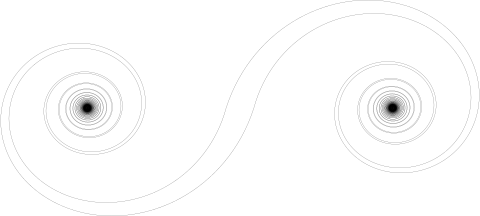
\includegraphics[scale=.625]{\figdir/plane-spirals.pdf}
    \caption{A ``Wild-Looking'' Curve in $\RR^2$}
    \label{fig:plane-spirals}
  \end{figure}
  Again: as can be seen from \cref{fig:two-gammas}, one can define
  this curve explicitly by applying a rotation to $\gamma_{0,1}(t)$,
  applying an appropriate shift, and adjusting the time scales to get
  agreement on the two boundary points. From
  \cref{thm:all-ambient-isotopic-in-r2}, it follows that this curve is
  ambient isotopic to the unit circle!
\end{example}
There's something strange going on at the centers of the spirals.
Namely, any line passing through them intersects the boundary of the
curve infinitely many times. For lack of a better name, we'll call
such points \emph{feral} points.\footnote{\emph{Feral} is chosen for
  its meaning as ``having escaped from domestication and become wild''
  (Merriam-Webster,
  \url{https://www.merriam-webster.com/dictionary/feral}). If a name
  for this concept already exists, or if the reader has a better
  suggestion for a name, please contact the author at
  \texttt{fkobayashi@g.hmc.edu}.} We'll draw a distinction here
between \emph{wiggly feral points} and \emph{swirly feral points} in
the definitions below. Note, in $\RR^2$, it might not be immediately
obvious why we would want to think of \emph{wiggly feral points} as
pathological at all, since they seem very easy to control. However, as
we'll see in $\RR^3$, points that look like \emph{swirly feral points}
when we take a projection into $\RR^2$ might turn out to be just
\emph{wiggly feral points} in another.
\begin{definition}[Wiggly Feral Point]\label{def:wiggly-feral}
  Let $K : S^1 \into \RR^2$ be an embedding. Let $s \in S^1$, and let
  $p = K(s)$. Reparameterize $K$ to be in polar form $r_p(t), \theta_p(t)$
  (for $t \in S^1$) such that the pole is at $p$. Then if there exist
  sequences $\pn{s_n}_{n \in \NN}, \pn{t_n}_{n \in \NN}$ such that
  \begin{enumerate}
    \item For all $n \in \NN$, $s_n \sprec t_n \sprec s_{n + 1}$, and
    \item At least one of the following holds:
      \begin{enumerate}
        \item For all $n \in \NN$,
          \[
          r_p(t_n) > \max\set{r_p(s_n), r_p(s_{n+1})},
          \]
          or
        \item For all $n \in \NN$,
          \[
          \theta_p(t_n) > \max\set{\theta_p(s_n), \theta_p(s_{n+1})}.
          \]
      \end{enumerate}
  \end{enumerate}
  Then we call $p$ a \emph{wiggly feral point} (sometimes just
  \emph{wiggly point}) of $K$. We say that $K$ is \emph{wiggly feral}
  or \emph{wiggly} at $p$.
\end{definition}
\begin{remark}
  This definition is meant to encode the idea that the graph of $K$
  ``oscillates'' infinitely often as we approach $p$. Note, this is
  quite different form our example in \cref{fig:plane-spirals}, where
  we actually have $\theta \incto \infty$. By contrast, \emph{wiggly
    feral points} are meant to capture behavior like the following:
  \begin{figure}[H]
    \centering
    \includegraphics[scale=.5]{\figdir/feral-point.pdf}
    \caption[Wiggly Arc]{An arc with a wiggly feral point.}
  \end{figure}
  \begin{figure}[H]
    \centering
    \includegraphics[scale=.5]{\figdir/smooth-countable-zigzag.pdf}
    \caption[Another Wiggly Arc]{A closed curve in $\RR^2$ with a
      wiggly feral point. We've drawn a tubular neighborhood around it
      just for pizzazz.
      % We'll look at this diagram again later when
      % we talk about tubular neighborhoods.
    }
  \end{figure}
  \begin{figure}[H]
    \centering
    \includegraphics[scale=.5]{\figdir/koch-snowflake.pdf}
    \caption[An Everywhere Wiggly Arc]{An everywhere-wiggly arc.
      Essentially every non-self-intersecting fractal is everywhere
      wiggly.}
    \label{fig:everywhere-wiggly}
  \end{figure}
\end{remark}
% \begin{remark}
%   Our definition of wiggly feral does not extend to curves that might
%   \emph{look} wiggly, but actually decay monotonically in both $\theta$.
%   \begin{figure}[H]
%     \centering
%     \includegraphics[scale=.75]{\figdir/wiggly-feral-problem.pdf}
%   \end{figure}
%   % We originally included \np{a condition similar to that on
%   %   $\theta_p(t)$} for $r_p(t)$, however, it appeared to us to be
%   % redundant.
%   % Our definition of wiggly feral appears not to cover situations where
%   % we have
% \end{remark}
% \begin{question}

% \end{question}
% We note some unresolved questions about this definition before
% continuing on to \emph{swirly} feral points.
% \begin{question}
%   Is this the best definition for wiggly feral? Are there cases when
%   we have very poorly-behaved $\theta(t)$ that don't have any local
%   optima but still ``oscillate'' wildly (maybe something not of
%   bounded variation, kind of like the Weirstrass function)?
% \end{question}
The case where $\theta \to \infty$ is covered by \emph{swirly feral
  points}.
\begin{definition}[Swirly Feral Point]\label{def:swirly-feral}
  Let $K : S^1\into \RR^2$ be an embedding. Let $s \in S^1$ be
  arbitrarily chosen, and let $p = K(s)$. Reparameterize $K$ to be in
  polar form $r_p(t), \theta_p(t)$ (for $t \in S^1$) such that the
  pole is at $p$. Then if $\theta_p(t) \to \pm \infty$ as $t \to s$,
  we say $p$ is a \emph{swirly feral point} (sometimes just
  \emph{swirly point}) of $K$. We say $K$ is \emph{swirly feral} or
  sometimes just \emph{swirly} at $p$.
\end{definition}
Sometimes it will be helpful to think of the swirly feral points
without needing to reparameterize. The following proposition gives one
way of doing so.
\begin{proposition}\label{prop:swirly-ferality-and-winding-number}
  Let $K : S^1 \into \RR^2$ be an embedding. Let $s \in S^1$ be
  arbitrarily chosen, and let $p = K(s)$. Consider an arbitrary
  infinite sequence of nested arcs $I_n$:
  \[
    \underbrace{\sbk{s_1, t_1}}_{I_1} \subseteq \underbrace{\sbk{s_2,
        t_2}}_{I_2} \subseteq \cdots \subseteq \underbrace{\sbk{s_n,
        t_n}}_{I_n} \subseteq \cdots.
  \]
  For each $n \in \NN$, define $\gamma_n$ to be the (possibly
  non-simple) curve defined by taking $\fim{K}{I_n}$ and connecting
  $K(s_i)$ and $K(t_i)$ with a straight line. Use $w_n$ to denote the
  winding number of $\gamma_n$ about $p$. Then $p$ is a \emph{swirly
    feral point} of $K$ iff there exists such a sequence of $I_n$'s
  such that
  \[
    \lim_{n \to \infty} w_n = \pm \infty.
  \]
\end{proposition}
\begin{remark}
  One should note that we require \emph{nested} arcs in the
  proposition above. The reason might not be immediately obvious: One
  can imagine a variety of swirly-looking curves that yield
  visually-similar graphs to \cref{fig:plane-spirals} but always
  ``double back'' before $w_n$ can get unbounded (we apologize for the
  lack of diagrams here). Why don't we want to include those? As it
  turns out, they are actually easier to treat, and are really better
  thought of as wiggly feral points.
\end{remark}
% \begin{remark}
%   One might note that both the definitions of \emph{wiggly-feral} and
%   \emph{swirly-feral} are tied to the local behavior of $\theta(t)$
%   close to the pole of some polar coordinate system, but only
%   \emph{wiggly-feral}. Why don't we see
%   similar pathologies in $r(t)$? Ultimately, this is by virtue of
%   continuity of $K$: $r(t)$ can be defined as ``for all $t \in S^1$,
%   $r(t) = d(p, K(t))$.'' Hence all of the bad behavior
% \end{remark}

One might wonder whether feral points have to obey some kind of
discreteness properties. This appears not to be the case, but we have
not investigated the matter in great detail. As a first example, note
that \cref{fig:everywhere-wiggly} is actually \emph{everywhere}
wiggly, hence we certainly can't expect discreteness from wiggly feral
points.\footnote{For an even more pathologically-flavored example, one
  might consider an \emph{Osgood curve}, which can actually have
  positive measure in $\RR^2$.} For swirly-feral points, the situation
is a bit trickier, but we propose the following counterexample to the
claim ``swirly feral points must be topologically discrete.''
\begin{counterexample}
  Let $K$ be defined iteratively from $K_n$ as follows.
  \begin{enumerate}
    \item Let $K_0$ be the spiral embedding from
      \cref{ex:swirly-feral-example}.
      \begin{figure}[H]
        \centering
        \includegraphics[width=5cm]{\figdir/plane-spirals-2.pdf}
        \caption{The spiral, redux}
      \end{figure}
    \item Draw a line through the center of the spiral:
      \begin{figure}[H]
        \centering
        \includegraphics{\figdir/swirly-sequence.pdf}
        \caption{A line through the centers}
      \end{figure}
    \item Define $K_i$ as follows: At each point of intersection $x_i$
      of the line with the spiral, $\fim{K}{S^1}$ locally looks like
      an arc. Hence, remove a small portion from $K$, and replace it
      with a shrunk-down copy of the spiral.\footnote{To guarantee the
      spiral will fit, we can apply \cref{thm:separating-strands}.}
      \begin{figure}[H]
        \centering
        \includegraphics{\figdir/swirly-replace.pdf}
        \caption[Replacement process]{A crude diagram for the
          replacement process. Unfortunately, \texttt{pgfplots}'s
          drawing capabilities gave out on us past the second
          replacment.}
      \end{figure}
      By applying uniform convergence, one can show that the limit of
      the $K_i$ is continuous.
  \end{enumerate}
  This gives an infinite sequence of swirly points converging to
  another swirly point. Hence we see the swirly points are not
  topologically discrete.
\end{counterexample}
We imagine that a similar construction can be used in a fractal-like
construction to yield a curve that is swirly feral on an uncountable
set. We leave some questions for future work:
\begin{question}
  Let $K : S^1 \into \RR^3$. Just how ``not discrete'' can the swirly
  feral points of $K$ be? E.g.,
  \begin{enumerate}[label=\arabic*)]
    \item Can the swirly points of $K$ be perfect?\footnote{Recall,
      perfect means ``closed and has no isolated points.''}
    \item Can the swirly points of $K$ be dense in
      $\fim{K}{S^1}$?
    \item Can the swirly points of $K$ have positive measure in
      $\fim{K}{S^1}$? (Here, we're viewing $S^1$ as $[0,2\pi]/\set{0
      \sim 2\pi}$ inheriting the Lebesgue measure on $[0,1]$).
    \item Can $K$ be swirly almost everywhere?
    \item Can $K$ be everywhere swirly feral?\qedhere
  \end{enumerate}
\end{question}
We have the following conjecture:
\begin{conjecture}
  The answers to the first three above are ``yes,'' ``yes,'' ``yes,''
  ``no,'' and ``no.'' Here's some of our intuition:
  \begin{enumerate}[label=\arabic*)]
    \item This seems fairly straightforward to accomplish by
      constructing a $K$ that maps a Cantor set to swirly feral points
      (e.g., identify the two loose ends of each sub-spiral with the
      endpoints of a Cantor set in $S^1$ and prove the
      correspondence).
    \item Here, one might try a construction that iterates through
      $\set{2\pi t \MID t \in \QQ \cap [0,1]}$ where the radii of our
      inserted sub-spirals decay according to the denominator of
      $t$.\footnote{This is basically Thomae's function but swirly.}
    \item Here, one might try the same argument as in (1) but with the
      Smith-Volterra-Cantor set.
    \item Our intuition is a bit shaky on these last two, but it seems
      that any construction for an ``almost everywhere swirly feral
      embedding'' would require the swirls to get small so quickly
      that in the limit, there's no winding about our points of
      interest. We'd be interested to see an example, though.
    \item If almost everywhere swirly feral fails, then so does
      everywhere swirly feral.
  \end{enumerate}
\end{conjecture}
This concludes our discussion of the 2D case. We now move into 3D,
where all the interesting pathologies lie.

%%% Local Variables:
%%% TeX-master: "../../kobayashi-thesis"
%%% End:
